% THIS IS SIGPROC-SP.TEX - VERSION 3.1
% WORKS WITH V3.2SP OF ACM_PROC_ARTICLE-SP.CLS
% APRIL 2009
%
% It is an example file showing how to use the 'acm_proc_article-sp.cls' V3.2SP
% LaTeX2e document class file for Conference Proceedings submissions.
% ----------------------------------------------------------------------------------------------------------------
% This .tex file (and associated .cls V3.2SP) *DOES NOT* produce:
%       1) The Permission Statement
%       2) The Conference (location) Info information
%       3) The Copyright Line with ACM data
%       4) Page numbering
% ---------------------------------------------------------------------------------------------------------------
% It is an example which *does* use the .bib file (from which the .bbl file
% is produced).
% REMEMBER HOWEVER: After having produced the .bbl file,
% and prior to final submission,
% you need to 'insert'  your .bbl file into your source .tex file so as to provide
% ONE 'self-contained' source file.
%
% Questions regarding SIGS should be sent to
% Adrienne Griscti ---> griscti@acm.org
%
% Questions/suggestions regarding the guidelines, .tex and .cls files, etc. to
% Gerald Murray ---> murray@hq.acm.org
%
% For tracking purposes - this is V3.1SP - APRIL 2009

\documentclass{acm_proc_article-sp}
\usepackage{balance}
\usepackage{graphicx}

\begin{document}

\title{Adaptive Monitoring using Openflow}
\subtitle{[Extended Abstract]}

\numberofauthors{3} 
\author{
\alignauthor
Author One\titlenote{sample titlenote}\\
       \affaddr{Institute One}\\
       \affaddr{Address One}\\
       \email{author.one@emails.com}
\alignauthor
Author Two\\
       \affaddr{Institute Two}\\
       \affaddr{Address Two}\\
       \email{author.two@emails.com}
%\and % go to new row
\alignauthor
Author Three\\
       \affaddr{Institute Three}\\
       \affaddr{Address Three}\\
       \email{author.three@emails.com}
%\alignauthor
%Author Four\\
%       \affaddr{Institute Four}\\
%       \affaddr{Address Four}\\
%       \email{author.four@emails.com}
}


\date{20 April 2013}

\maketitle

\balance

\begin{abstract}
This paper present a network monitoring architecture which take advantages of Software Defined Network and traditional monitor methods. Our architecture support the a number of features: 1)monitoring both large and small flows with low cost, 2)adjust the work condition automatically according to the flow status, 3)accept instructions from users and other applications to control the flow, 4)combined with traditional detection methods.

optional: 1)support long-term flow analysis...
TODO: make features clearly
\end{abstract}

% A category with the (minimum) three required fields
%\category{H.4}{Information Systems Applications}{Miscellaneous}
%A category including the fourth, optional field follows...
%\category{D.2.8}{Software Engineering}{Metrics}[complexity measures, performance measures]

\terms{Application}

\keywords{network monitor, openflow} % NOT required for Proceedings


\section{Introduction}
In modern datacenters, collecting the network flow statistics information and DPI information is important for attack detection and resource allocation. By monitoring the network flows, we could know whether there's irregular flows, which part is the most active and when to upgrade the whole system. If the bandwidth demands of servers and applications are changing dynamically, it is too difficult to give reasonable predictions and only real-time monitoring is feasible.\\
However, the procedure of monitor all the network flows usually cost too much and we have to make a compromision between efficiency and accuracy.\\ 
(TBA) More details\\
(TBA)Our main contribution.\\
\\
\\
\\


\section{Related Work}
(TBA)Related Work\\
Sample Citation:\\
openflow: \cite{openflow-2511}\\
B4: \cite{google-b4-225}\\
csamp: \cite{csamp-97}\\

The structure of the rest of this paper.

\section{Our Method}
(TBA)Brief summary of related work. Discuss the advantages and disadvantages of Sample, Mirror and so on.\\
(TBA, motivation)Now we consider the cost when we try to get the network flow information. If we use openflow table to monitor an point-to-point flow, the cost is one flow entry. If we mirror a flow to a server, the cost is the bandwidth. In our system, we use openflow entry to monitor large flow, and mirror small flows to the server.\\
The rest of the sections is arranged as follows. The system architecture part described the hardware architecture and flow table design, and why we build our system like this. The flow bandwidth monitor describes the algorithm and feedback control on filtering large flows and monitor small flows. The ddos attack detection describe how to monitor long-term ddos attack as well as short-term attack. The deep packetage information detection describe how we detect the package content by using other tools. And the operation for uses command part describe how can we follow users' instructions.\\

\subsection{System Architecture}
Hardware Structure

(image)\\
             user --> controller\\
             controller <--> switch\\
             switch ---> servers\\
             switch --> mirror server\\
             switch --> snort node(third-part tools)\\
             mirror server --> controller\\
             snort node --> controller\\
             (add port information, and link to controller is inband)\\


Briefly introduce the structure of different part and their relationships.\\
Briefly intrudoce the detailed structure of the controller.\\
Flow table Struction:\\
(image)\\
            flow table 1:\\
            ~~~~ for high level monitor (user different priority)\\
            flow table 0:\\
            ~~~~ for determinate flow monitor while can make routing decision by oneself (high priority)\\
            ~~~~ fow learning switch(low priority), inlucding the lowest priority packet-in\\

(TBA)Explain why use the high level part to monitor and routing, but not add another table. (Due to the hardware implentation of multi-table on Pica8...--Can we write like this?--)\\
(TBA)Explain why use table one for high level monitor. (It can't make routing decisions by one self. eg. all flow come from a given IP.)\\

\subsection{Flow Bandwidth Monitoring}
Bandwidth Detection:\\
Use flow entris to filter elephant flow.\\
Use feedback to adjust monitoring entries. If the mirror bandwidth extend the port bandwidth, times the factor for feedback result\\
\\
Flow Entry Replacement Algorithm\\
All use generated flow matrix to test. Easy to reappear.\\
Random vs Greedy vs Damping using long-term history and dft\\
compare target: mirror bandwidth,  monitor precision, entry change time and so on.\\
Use dft to detect whether the flow is mutable or stable. Combine it with the average flow size to determine whether to add the corresponding monitor entry.\\
Store long-term information also help to ddos detection.\\

\subsection{DDos attack detection}
Store all the flow statistics information of a period time.\\
For each src node and dst node, use the relavent flows to determine whether it is a potential attacker or a target.

\subsection{Deep Package Information Detection}
The shortage of our SDN monitor is we can't look up into the packets on the switch. Even we can look into the information in a packet when packet-in event happens, we can't affort the cost of packet-in. A general controller could only deal with 1k-10k packet-in request, which we will test later.\\
snort

\subsection{Operation for User Command}
Monitor Flows, Block Ports\\
Change work status.\\


\section{Evaluation}

\subsection{Environment Setup}
Hardware parameters introduction. Pica8-3295 and server models\\
Real System connection struction.\\

\begin{figure}[htbp]
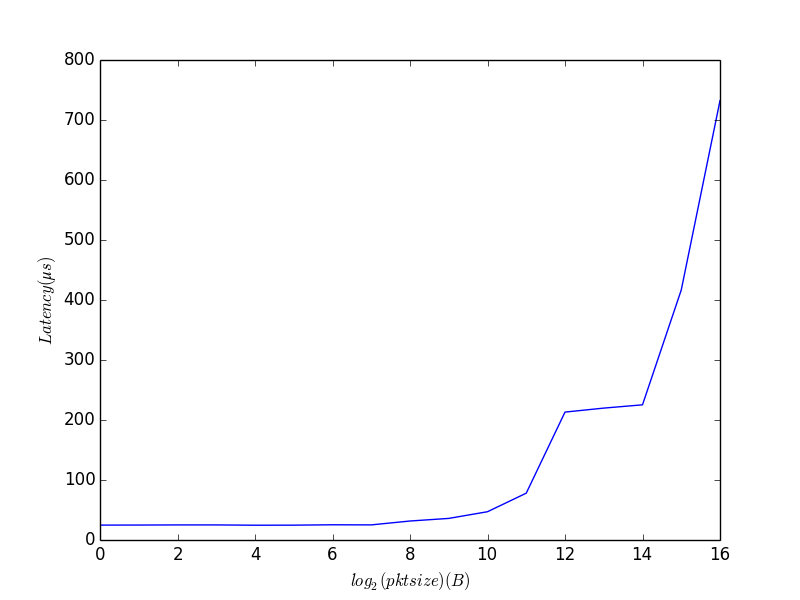
\includegraphics[width=3in]{image/latency}
\caption{Latency-L2}\label{fig:latency-l2}
\end{figure}
\begin{figure}[htbp]
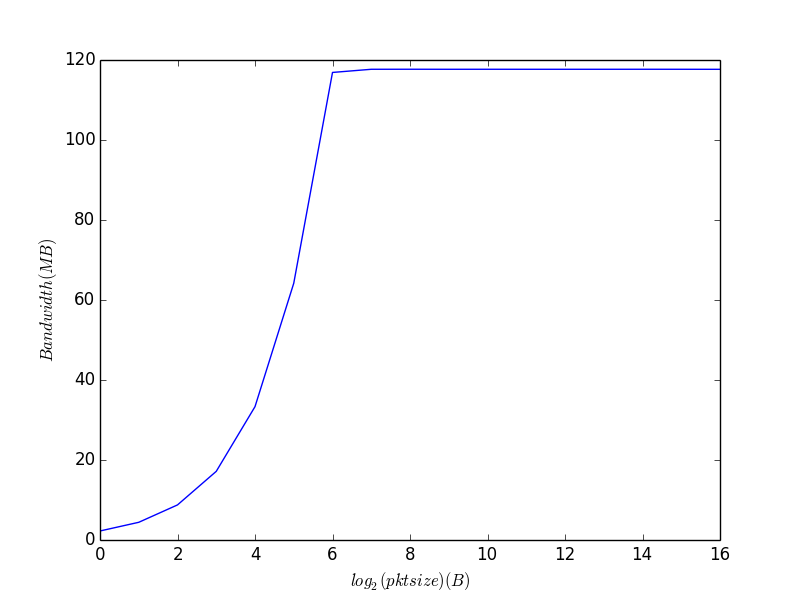
\includegraphics[width=3in]{image/bandwidth}
\caption{Bandwidth-L2}\label{fig:Bandwidth-l2}
\end{figure}

(Test is based on the features our method support, and including performance test.)

\subsection{Basic Environment Test}
Test on Switch and Controller:\\
Basic Test.\\
Use cbench or other tools. Test on standard learning switch between our switch.\\
(optional)Test the basic parameters of our system.

\subsection{Compared with L2}
Compare the Bandwidth and Latency under L2 and Openflow:\\
use scripts (got help from liyiran)\\
Test bandwidth between servers under L2 model and Openflow model. If these's little difference, change it to the test between L2 and openflow with our controller\\
(image)\\
Test bandwidth between servers under Openflow model with insert/delete monitor flows on different frequency.\\
(image)\\

Test the Bandwidth and Latency influence of inserting and deleting monitor flows.\\
Also test whether it lead to packet-loss when insert and delete flow entries.\\

\subsection{Precision}
Bandwidth(Elephant FLow):\\
Compared with sFlow.\\
Use generated flows, Compare the precision.\\
When bandwidth is not full, when mirror port is full.\\
absolute precision, precision compared with sflow.

DDoss:\\
Compared with?
absolute precision
long-term feature
react time

\subsection{Reaction Time}
The attack start time and detected time
DPI
user's command

\subsection{Cost, Cost includes flow entry, mirror bandwidth}
Use generated flows\\
Use real cluster flows(eg. Spark). Depends on the flow characteristc.


\section{Conclusion}
Conclusion\\


\bibliographystyle{abbrv}
\bibliography{sample}

\end{document}
